\subsubsection{UC19 - Leaderboard}
\begin{figure}[h]
	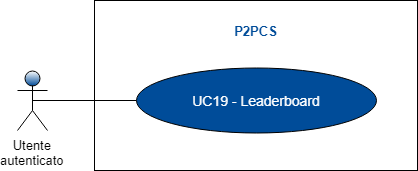
\includegraphics[width=9cm]{res/images/UC22Leaderboard.png}
	\centering
	\caption{UC19 - Leaderboard}
\end{figure}
\begin{itemize}
	\item \textbf{Attori Primari}: utente autenticato;
	\item \textbf{Descrizione}: attraverso un'apposita sezione dell'area personale, l'utente può visualizzare la classifica dei migliori utenti, i quali vengono classificati in base ai punti esperienza totali in loro possesso. Al termine di un periodo prestabilito, i primi tre utenti della classifica riceveranno un premio che può consistere in:
	\begin{itemize}
		\item punti esperienza bonus;
		\item accessori per personalizzare l'auto nel Minigioco;
		\item sconti su spesa o e-commerce;
		\item un viaggio gratis con \textit{GaiaGo}.
	\end{itemize}
	la Leaderboard mostrerà per ogni utente:
	\begin{itemize}
		\item la posizione;
		\item il nome e cognome dell'utente;
		\item il totale dei punti esperienza.
	\end{itemize}
	\item \textbf{Scenario principale}: l'utente preme il pulsante \textit{Leaderboard} e consulta la classifica utenti;
	\item \textbf{Precondizione}: l'applicazione rende disponibile la visualizzazione della Leaderboard\glo;
	\item \textbf{Postcondizione}: l'utente autenticato ha visualizzato la Leaderboard.
\end{itemize}

